% !TEX root = HowToRobot.tex

\chapter{Mechanical Design}
\label{chap:MechDes}

\section{Design Considerations}
One hugely important aspect of your robot design is ensuring it is mechanically capable of fulfilling requirements - and making sure it doesn't collapse under its own weight. No amount of sophisticated code, nor the most powerful computer in the world, can force your robot to function if the chassis is compromised. It is tempting - we fell in to this trap several times during my time on the Robotics Team - to want to design your perfect robot from the ground up. Don't. If this is your first robot, or even second or third, take my word for it and just buy a chassis.

Seriously.

Mechanical design is time-consuming and, unless you have several skilled mechanical designers around, likely going to be difficult. On the Mines campus, it has become increasingly difficult to do any real fabrication, thanks in part to the increasingly strict attention to safety, and the CAT lab's understandable desire to cut down on machining costs.\\

Going for it anyway? Good for you, however, keep a few things in mind:

First, keep it simple. Complex designs are more expensive, have tighter tolerances, take a great deal longer to design and fabricate, and - most importantly - have more ways to fail. The best design in the world is useless if it never makes it off paper.

Second, keep moving parts to a minimum. This is similar to point one, but it's important enough to say twice. Every moving part means you need to deal with routing power i.e. keeping cables from getting tangled. Every moving piece also generally adds weight, cost, and complexity.

Third, if the words "we'll attach this here somehow" are ever uttered, take a closer look. We like to think in the CSC department that Mechanical Engineering is just hitting things with hammers and turning wrenches, but building real things is actually very difficult. Every piece of your robot has to be attached somehow - avoid glue - and that's not something that just sorts itself out once you have all the pieces.

Fourth - No, hot glue is not a good idea. Trust me. Been there. It's not. Epoxy can work, but it's no substitute for bolts.

Fifth - 3M velcro tape is better, but still not good, and is only appropriate for an indoor non-competition research vehicle where frequent reconfiguration is expected. See the SMP and Mecanum chassis for examples. It doesn't hold up under vibration as well as you would think. It holds great against normal stress, but not terribly well against sheer stress, and not at all against twisting stress.

Sixth, iterate. Don't expect your first build to be perfect. In all honesty, it probably won't even work. You forgot something or overlooked something or assumed something that isn't right. I promise. Give me a call before you start designing, and I will bet you \$100. Expect your design to fail, and get something built as early as possible. A failed design isn't the end of the world unless it's the day of competition. More than one of our designs failed because we were half-way into the spring semester before we got anything built, and there was no time to try again.

Seventh, failure is good. You learn a whole lot from mistakes. Don't be afraid to try something just because it might not work. It \textit{definitely} won't work the first time anyway.

\section{Requirements}

What does your robot need to do? Agile development is great for software, and there are some applications that can be adapted to hardware, but you really need to know what you're getting into before you start buying or building things. I can't possibly predict every possible requirement, but here are a few important ones I have come across before.

How does the robot need to move? Whether mobile or fixed, your robot likely needs to actuate within its workspace, and this will be one of the main factors in the mechanical design.This will be addressed further in section \ref{section:kinematicModels}.

How fast does the robot need to be? If your robot doesn't need to be very fast, you can reduce power requirements, use smaller and/or cheaper motors, and you don't have to worry as much about vibrations. If the robot needs to be fast, the inverse is true.

How strong does the robot need to be? If the robot only needs to drive from A to B on a card table carrying a few paperclips, an Arduino taped to a few continuous rotation servos and some cardboard will probably do the trick. If you need to carry a cinderblock around an outdoor obstacle course, you need a robust frame, bigger motors, bigger batteries, and space to put it all.

How durable does the robot need to be? This one is pretty self-explanatory. However, keep in mind that as soon as you have a working RC robot, people will want to play with it. They will crash it. Hard. Once the robot is driving autonomously, it will crash itself. Often \textit{and} hard. Make sure all potential contact surfaces on the robot can survive impact at maximum speed with something sharp and/or hard.

Does it need to be waterproof or water-resistant? Some competitions - like the Sparkfun AVC - are outdoors. Given Murphy's law, this means it will probably rain. Plan early about ways to keep water out and the magic smoke in. Never put holes in the top, and consider rubber grommets or seals around connectors and cabling. Also consider having angled non-porous surfaces on the top of the robot to deflect water such that it will drip harmlessly away from the electronics.

Does it need to be heat-tolerant? This, unfortunately, is in direct conflict with being waterproof, because you need to put holes in the robot for air circulation. We never came up with a perfect solution that handles both. Assume your CPU, GPU (if you have one), motor controller, and motors will attempt to melt anything in contact with them as soon as you close the case. Make sure you have proper heat-sinking and, if possible, forced air-flow over those heat-sinks. Also make sure the air has a way to escape. If operating outdoors, make sure you have filtered air intake.

Finally, what does it need to do? Claws, grippers, baskets, sensors, and payloads all need secure mounting. Make sure you include some sort of mounting bracket for whatever tools your robot will need to complete its job.

\section{Kinematic Models}\label{section:kinematicModels}

Now that you know what your robot needs to do, it's time to actually start designing something. For a mobile robot, kinematics are everything. There are a few common kinematic models that I want to cover in some detail.

Each kinematic model has different advantages and disadvantages, so it is important to consider how your robot needs to be able to move before selecting one.

\subsection{Differential Drive}

The simplest and most common drive system for a mobile robot is differential drive. This involves a fixed axle with two independently driven motors at the ends. A picture is worth a thousand words, so check out Figure \ref{fig:diffdrive}, borrowed from the nice people at www.robotplatform.com.

\begin{figure}[h]
\centering
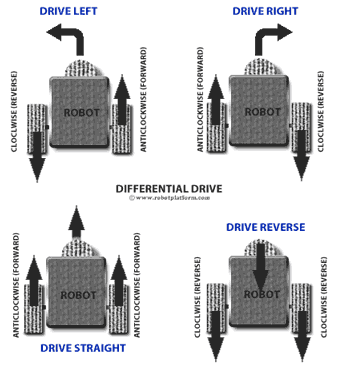
\includegraphics[width=0.6\textwidth]{Differential_Drive.png}
\caption{Differential Drive}
\label{fig:diffdrive}
\end{figure}

Differential Drive is very simple because it only requires two powered wheels. In the image, the front wheel is a caster wheel, or a skid-pad, and is only present to keep the robot upright.

One major advantage of the differential drive paradigm is the ability to turn in place by spinning one wheel forward, and one back. However, because of the skid-pad or caster wheel, differential drive is typically only used in low-speed applications. The extra drag and wobbling of an uncontrolled wheel could cause vibrations or instability at high speeds.

%I won't go into the derivation of the kinematic model, but I will present it here so you can use it for reference. There %are two kinematic models of interest, the forward kinematic model and the inverse.

%The reverse kinematic model tells you how the robot will move given a set of wheel velocities, and is shown in Equation %\ref{eqn:diffdriveforward}.

%TODO: Add kinematics?

\subsection{Ackermann Drive}

Ackermann drive is a common choice for high speed robots because it provides better stability and less drag than the differential drive. It is also the same steering system that most cars use. However, an Ackermann steered vehicle cannot turn in place.

An Ackermann drive vehicle must have two front wheels which can be turned, and two fixed rear wheels. It is common to have powered rear wheels since the pivoting front wheels adds additional complexity when attempting to mount motors, but powered front wheels are not unheard of. See Figure \ref{fig:ackermann}.

\begin{figure}[h]
\centering
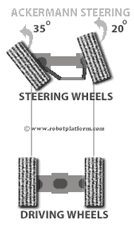
\includegraphics[width=0.25\textwidth]{Ackermann_Drive2.png}
\caption{Ackermann Drive}
\label{fig:ackermann}
\end{figure}

There is one additional complication to consider when attempting to build your own Ackermann Drive system. When an Ackermann vehicle turns, each wheel is essentially drawing out the circumference of a circle. To take that thought a step further, both steering wheels will be drawing out circles, but of slightly different radii - the difference being the center to center distance from wheel to wheel. Therefore, to avoid wheel slip while drawing two circles of different sizes, each wheel must be at a slightly different angle. The difference changes depending on how sharp of a turn is desired. Obviously designing a mechanical system to automatically handle this would be complex, and writing code to handle turning each wheel individually would be non-trivial at best. I will once again recommend buying a professionally made drive system over building one unless you have a really good reason not to.

%TODO: Add kinematics?

\subsection{Skid Steer}
\label{sec:skidsteer}
Skid Steer A.K.A. Tank Drive, is another common form of locomotion. It's similar two having two differential drive systems mounted with a rigid bar between them. See Figure \ref{fig:skid_steer_drive} for an example of how Skid Steer drives. Each side, regardless of how many wheels it has, is unified, meaning that all wheels on the left drive at the same time and speed, as do all the wheels on the right. Tank drive is arguably better for an outdoor robot because it is much harder to end up high-centered when all of your wheels are powered. This also gives you more traction. However, to do anything other than drive straight forward or backward, some of the wheels have to slip. The largest disadvantage to Skid Steer is that any sort of wheel speed or encoder based odometry becomes very unreliable.

\begin{figure}[h]
\centering
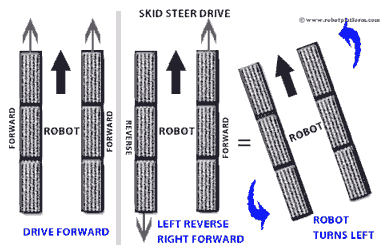
\includegraphics[scale=0.7]{skid_steer_drive.png}
\caption{Skid Steer}
\label{fig:skid_steer_drive}
\end{figure} 

However, if you have some other means of localization, like the LIDAR on the SMP robots, or the ASUS RGBD sensor, this becomes less of a problem. You end up with less drag than traditional differential drive and potentially more power because each wheel may (but doesn't have to) have its own motor. In addition, this design is much simpler to implement than Ackermann Steering or Omni-Drive, which will be discussed next. For these reasons, the SMP robots use Skid Steer. See the SMP in Figure \ref{fig:smprobot}.

\begin{figure}[h]
\centering
\includegraphics[width=.7\textwidth]{smprobot.png}
\caption{SMP Robot}
\label{fig:smprobot}
\end{figure} 

\subsection{Omni-Driv}

An Omni-Drive robot is one that can move in any direction. There are several ways to construct an Omni-Drive robot, but I will focus on a four wheeled robot with fixed wheels in "traditional" positions. The Mecanum robot shown in Figure \ref{fig:mecanumrobot} - named so for the style of wheels - is one such robot.

\begin{figure}[h]
\centering
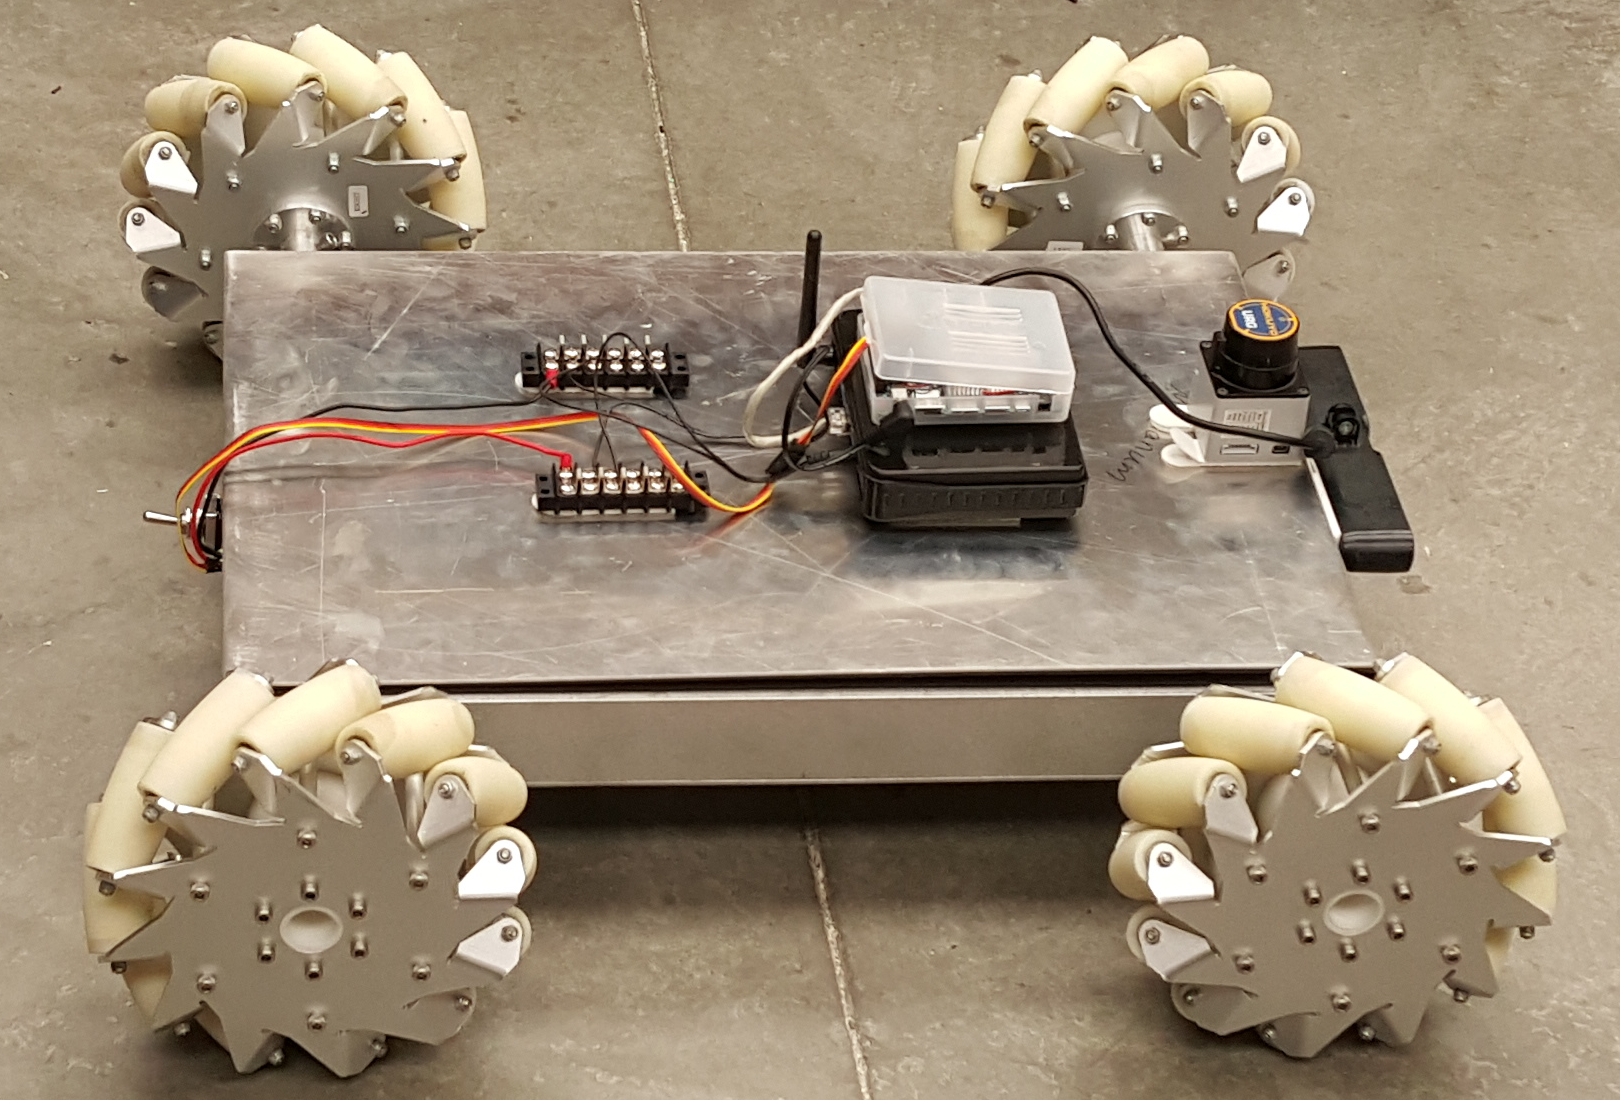
\includegraphics[width=.65\textwidth]{mecanumrobot.png}
\caption{Mecanum Robot}
\label{fig:mecanumrobot}
\end{figure} 

%\begin{figure}
%\centering
%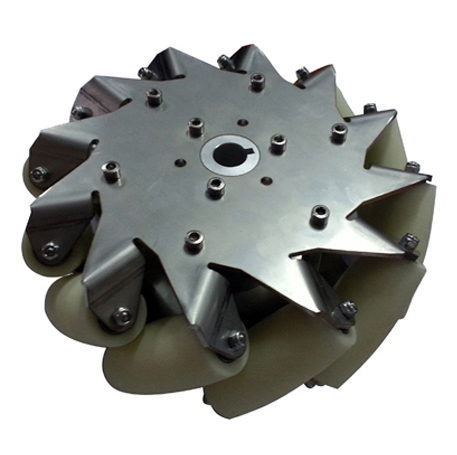
\includegraphics[width=0.45\textwidth]{mecanumwheels.png}
%\caption{Mecanum Wheel}
%\label{fig:mecanumwheels}
%\end{figure} 

Omni-Drive kinematics are complex, but I will attempt a brief summary. The rollers on this style of mecanum wheel are mounted at 45 degrees. The means that of any amount of force applied to rotating a wheel, only approximately half will be exerted along the line parallel with the direction of travel. The other half will be exerted along the perpendicular axis. The wheels are not mounted symmetrically, however. All wheels are mounted such that, if all wheels turn forward, the perpendicular forces will cancel, allowing the robot to move forward. By operating the wheels in opposing pairs, a force in any direction can be generated, allowing the robot to translate and rotate in any direction freely. Figures \ref{fig:mecanumlocomotion} shows examples of the motion generated by various combinations of wheel speeds. This is very useful for a robot, because it means there aren't any constraints that have to be considered when attempting to operate the robot autonomously. If you want to move in a certain way, you can, no questions asked.


\begin{figure}
\centering
\begin{subfigure}{.5\textwidth}
  \centering
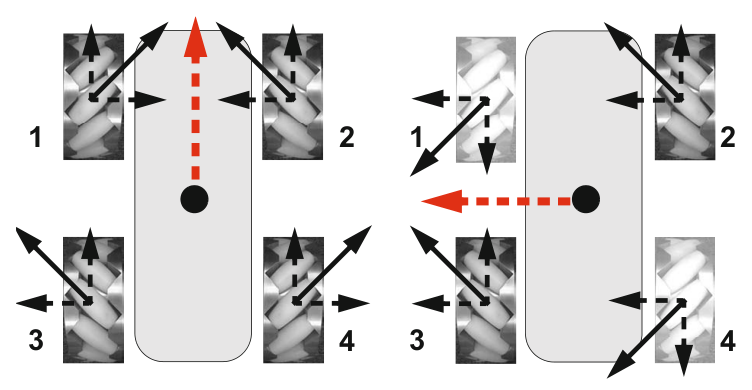
\includegraphics[width=\textwidth]{swedish_vector2.png}
  \caption{Translation}
  \label{fig:sub1}
\end{subfigure}%
\begin{subfigure}{.5\textwidth}
  \centering
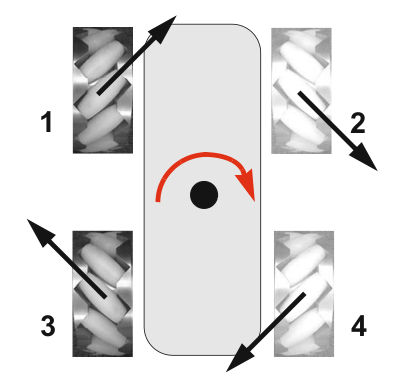
\includegraphics[width=.5\textwidth]{swedish_vector3.png}
  \caption{Rotation}
  \label{fig:sub2}
\end{subfigure}
\caption{Mecanum Locomotion}
\label{fig:mecanumlocomotion}
\end{figure}

While the actual mathematics for driving an Omni-Drive robot are relatively complex, the concept is simple. Just calculate the translation you want to preform, then the rotation, and add them. In this case, the total is just the sum of the parts. Special care should be taken, however. Attempting to both drive forward and turn at full speed works fine mathematically, but once you command a wheel to drive faster than its top speed, the robot will begin to behave erratically as the forces will no longer properly cancel.



























